\documentclass[11pt,a4paper]{article}
\usepackage[utf8]{inputenc}
\usepackage[T1]{fontenc}
\usepackage{amsmath}
\usepackage{amssymb}
\usepackage{amsfonts}
\usepackage{graphicx}
\usepackage[spanish]{babel}
\usepackage{booktabs, fourier, tabularx, wrapfig, multicol,multirow,caption, subcaption,tikz, fancyhdr, steinmetz, xcolor}
\usepackage{xfrac}
\usepackage[many]{tcolorbox}

\usepackage[left=2cm,right=2cm,top=2cm,bottom=2cm]{geometry}

\graphicspath{{./img/}}

%Acá voy a probar la rama
%%Acá va la segunda parte

%Configuración y comandos

%tcolorbox personalizado
\newtcolorbox{cajita}{colback=white!97!brown, colframe=brown!15!gray, breakable}

%Encabezado y pie de página
\fancyhead[R]{\textsc{Máquinas Eléctricas}}
\fancyhead[L]{
\includegraphics[width=.1\textwidth]{utncom}}
\fancyhead[C]{Hoja de fórmulas}
\fancyfoot[R]{ \vspace{.1cm} Página \thepage }
\fancyfoot[L]{\hrule \vspace{.1cm} Ingeniería Electromecánica}
\fancyfoot[C]{ \vspace{.1cm}}

\newtcolorbox{mybox}[1]{title = \textsc{Unidad #1},colbacktitle=red!85!black,enhanced,attach boxed title to top center={yshift=-2mm}, colbacktitle=white, coltitle=gray!50!black, boxed title style={colframe=blue!30},colback=white!97!brown, colframe=blue!30}

%Comando para fasores :)
\newcommand{\fasor}[1]{\uppercase{\textbf{#1}}}
%Comando título de cada unidad
\newcommand{\unidad}[2]{\begin{center}
		\fontsize{10}{10}\selectfont\color{gray!50!black}\scshape Unidad #1 \\
		\fontsize{14}{14}\selectfont \scshape #2
	\end{center} \vspace{-.6cm}}
%Comando para subtitulos
\newcommand{\subtitulo}[1]{
	\textbf{#1} \\ \vspace{.1cm} {\color{gray} \hrule}
}
%Comando para subsubtitulos
\newcommand{\subsubtitulo}[1]{
	\begin{flushleft}
		\vspace{.1cm}
		\textsc{#1}
		\vspace{.1cm}
	\end{flushleft}
}

\begin{document}
	\pagestyle{fancy}
	\section*{Nomenclatura}
	
	\begin{tabular}{r l r l}
		$\fasor{Z}$ [$\Omega$]& Impedancia &
		$\fasor{i}$ [A] & Corriente \\
		$\fasor{v}$ [V] & Tensión&
		$j$ & Unidad imaginaria \\
		$t$ [s] & Tiempo &
		$P$ [W] & Potencia activa \\
		$Q$ [VAr] & Potencia reactiva &
		$\fasor{s}$ [VA] & Potencia aparente \\
		$m$ & Relación de transformación&
		$\fasor{I}_{exc}$ o $\fasor{I}_0$ [A] & Corriente de excitación\\
		$\fasor{I}_{Fe}$ [A] & Corriente debido a pérdidas en el Fe&
		$\fasor{I}_{\mu}$ [A] & Corriente magnetizante\\
		$\fasor{v}_0$ [V] & Tensión en vacío & $\fasor{v}_{pc}$ [V] & Tensión a plena carga \\
	\end{tabular}
	\unidad{1}{Acá quiero poner lo de las bobinas y eso... VER}
	\unidad{2}{Transformadores}
	
	\begin{cajita}
		\centering
		
		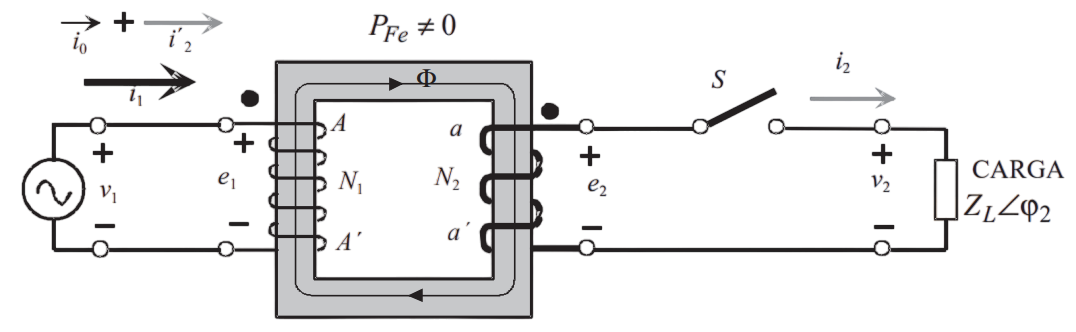
\includegraphics[width = .8\linewidth]{carga-trafo}
		\begin{multicols}{2}
		
			\begin{center}
				\subtitulo{Transformador Ideal \textnormal{en vacío} \vspace{.1cm}} 
			\end{center}
			
			\subsubtitulo{sin pérdidas en el núcleo de Fe} 
			
			\begin{tabular}{l l}
				Autoinducción & $L = \dfrac{\mu N^2 S}{l}$ \\
			\end{tabular}
		
			\subsubtitulo{con pérdidas en el núcleo de Fe}
			
			\begin{tabular}{l l}
				Fem & $\mathcal{F} = N_1  \fasor{i}_1  = N_1  \fasor{i}_0$\\
				Relación de transfor. & $m = \dfrac{E_1}{E_2} = \dfrac{N_1}{N_2}$ \\
				\multicolumn{2}{c}{$ \fasor{i}_0 = \fasor{i}_\mu + \fasor{i}_{Fe} $} \vspace{.1cm} \\ 
				\multicolumn{2}{c}{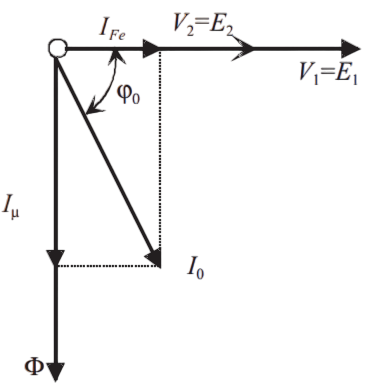
\includegraphics[width = .5\linewidth]{vacio-fasores}} \\
			\end{tabular} 
		
	
			\begin{center}
				\subtitulo{Transformador Ideal \textnormal{en carga}}
			\end{center}
		
			\vspace{-.6cm}
			
			\subsubtitulo{con pérdidas en el núcleo de Fe}
		
			\begin{tabular}{r l}
				Fem & $\mathcal{F} = N_1  \fasor{i}_1 - N_2 \fasor{i}_2$\\
				& $\mathcal{F} = N_1 \fasor{i}_0$\\
				& $\fasor{i}_0 = \fasor{i}_1 - \dfrac{N_2}{N_1} \fasor{i}_2$\\
				Corriente reducida & $\fasor{i'}_2 = \dfrac{\fasor{i}_2}{m}$ \\
			\end{tabular}
		
		\end{multicols}
	
	\newpage
	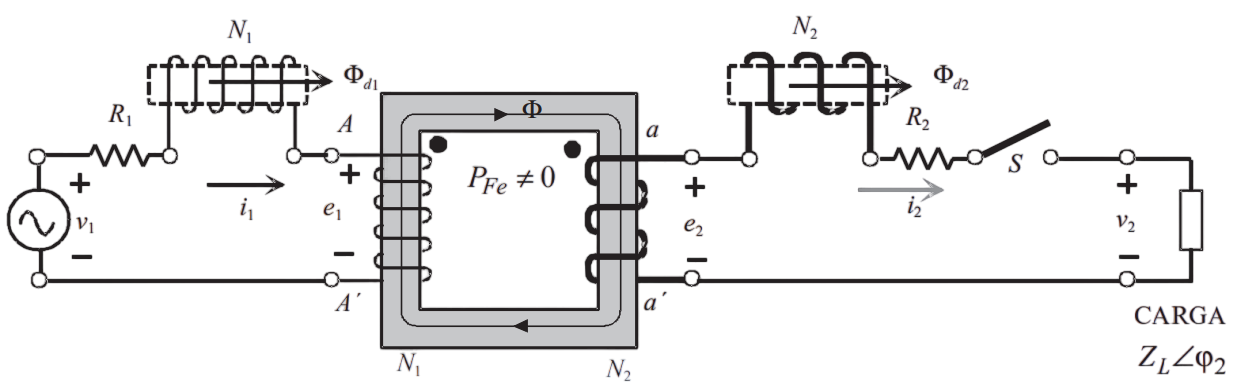
\includegraphics[width = .8\linewidth]{trafo-real}
	
	\begin{multicols}{2}
	
	\begin{center}
		\subtitulo{Transformador Real \textnormal{en vacío} \vspace{.1cm}}
	\end{center}
	
		\begin{tabular}{l l}
			$\fasor{v}_1 = \fasor{e}_1 + R_1 \fasor{i}_0 + j X_1 \fasor{i}_0$ & $\fasor{v}_{20} = \fasor{e}_2$ \\
			En trafos industriales & $m \approx \dfrac{V_1}{V_2}$\\
		\end{tabular}\\
	
		\begin{center}
			\subtitulo{Transformador Real \textnormal{en carga}}
		\end{center}		
		
	\end{multicols}
	
	\subtitulo{Circuito equivalente aproximado}
	
	\begin{flushleft}
		Se muestra el circuito referido al primario. Cuando es referido al secundario se hace un análisis similar.
		
		La \textsl{rama paralelo} siempre permanece del lado de alta tensión.
	\end{flushleft}

	\begin{multicols}{2}
		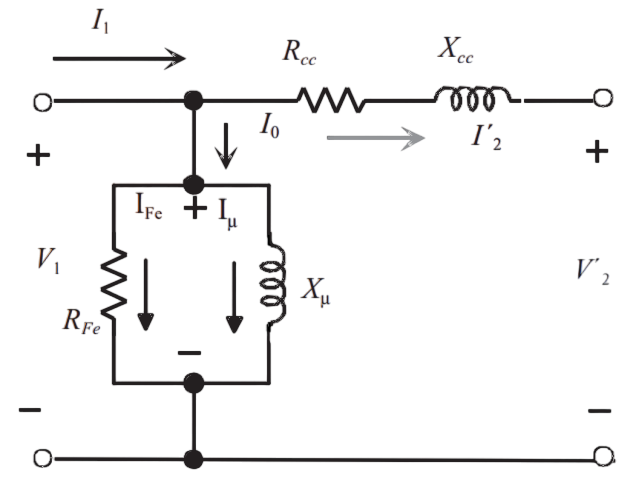
\includegraphics[width=.8\linewidth]{equi-aprox} \\
		
		\begin{tabular}{l l}
			Resistencia de cortocircuito &
			$R_{cc} = R_1 + R_2'$\\ \vspace{.1cm}
			Reactancia de cortocircuito & $X_{cc} = X_1 + X_2'$ \vspace{.2cm}  \\
			\multicolumn{2}{l}{\textbf{Parámetros referidos al primario} \vspace{.1cm}} \\ \vspace{.1cm}
			Número de espiras & $N_2' = m N_2$ \\ \vspace{.1cm}
			Tensión referida & $V_2' = m V_2$ \\ \vspace{.1cm}
			Corriente referida & $I_2' = \dfrac{I_2}{m}$ \\ \vspace{.1cm}
			Impedancia referida & $Z_2' = m^2 Z_2$ \\ \vspace{.1cm}
			& $Z_2 = R_2 + j X_2$\\
		\end{tabular}
	\end{multicols}
	
	\begin{multicols}{2}
	\subtitulo{Ensayo de vacío}	
	
	
		\begin{flushleft}
			Permite determinar las pérdidas en el $Fe$
			y los parámetros de la rama paralelo, $R_{Fe}$ y $X_\mu$.
		\end{flushleft}
	
			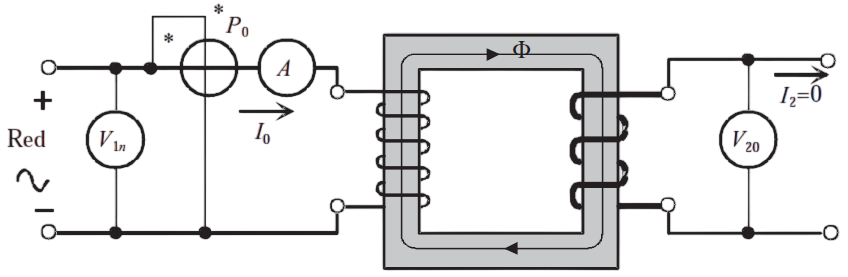
\includegraphics[width=\linewidth]{ensayo-vacio}\\ \vspace{.3cm}
			
			
			\begin{tabular}{c c}
					Pérdidas en Fe & $P_0 = P_{Fe} = V_{1n}\cdot I_0 \cos \phi_0$\vspace{.3cm} \\ 
					$ R_{fe}=\dfrac{V_{1n}}{I_{0} \cos \phi_0} $ &$X_{\mu}=\dfrac{V_{1n}}{I_{0}\sin \phi_0}$\\
			\end{tabular}\\
		
%			Se puede determinar la correspondencia entre las bobinas:\\
%			$\bullet$ A corresponde con y si: $V_{3}=V_{1}+V_{2}$\\
%			$\bullet$ A corresponde con x si: $V_{3}=V_{1}-V_{2}$\\
			
			\newpage %Similar al columnbreak pero deja alineado todo hacia arriba y no intenta distribuir en el eje y
			
	\subtitulo{Ensayo de cortocircuito}
		
		\begin{flushleft}
			Permite determinar las pérdidas en el $Cu$ y los parámetros de la rama de cortocircuito,  $R_{cc}$ y $X_{cc}$. $\fasor{I}_{0}$ es despreciable.
		\end{flushleft}
		
			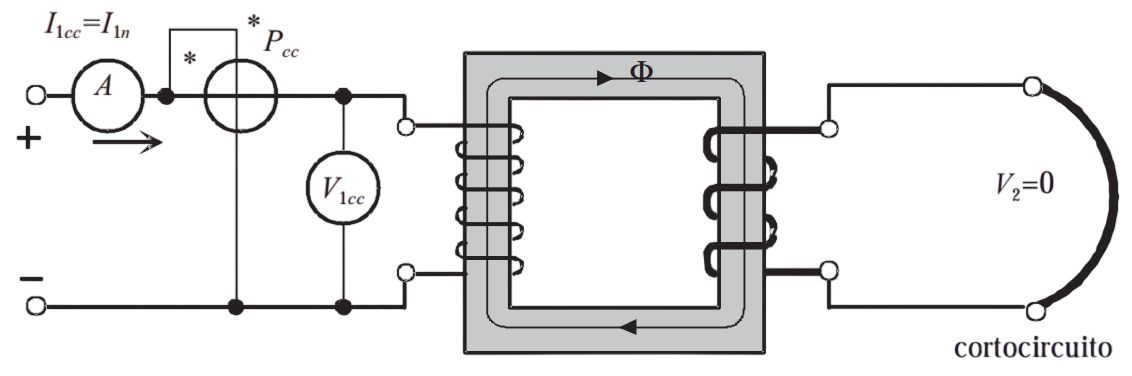
\includegraphics[width=\linewidth]{ensayo-cc}\\ \vspace{.1cm}
			
				
			\begin{tabular}{c c}
				\multicolumn{2}{c}{$P_{cc} = P_{Cu} =V_{cc}\cdot I_{1n} \cos\phi$}\\[0.1cm]
				$ R_{cc}=\dfrac{V_{1cc}}{I_{1n}} \cos\phi_{cc} $ &$X_{cc}=\dfrac{V_{1cc}}{I_{1n}} \sin\phi_{cc}$\\[0.4cm]
				
%							$\fasor{I}_{fe}=\fasor{I}_{0}.Cos[\phi_{0}] $& ; & $\fasor{I}_{\mu}=\fasor{I}_{0}.Sin[\phi_{0}] $\\[0.2cm]
			\end{tabular}
			
	\end{multicols}
	En ambos ensayos, los factores de potencia $\cos \phi_{0}$ y $\cos \phi_{cc}$ son las incógnitas a determinar para calcular los parámetros.
	
		\newpage
		
		\subtitulo{Regulación de Voltaje}
		\vspace{.3cm}
		
		\begin{multicols}{2}
			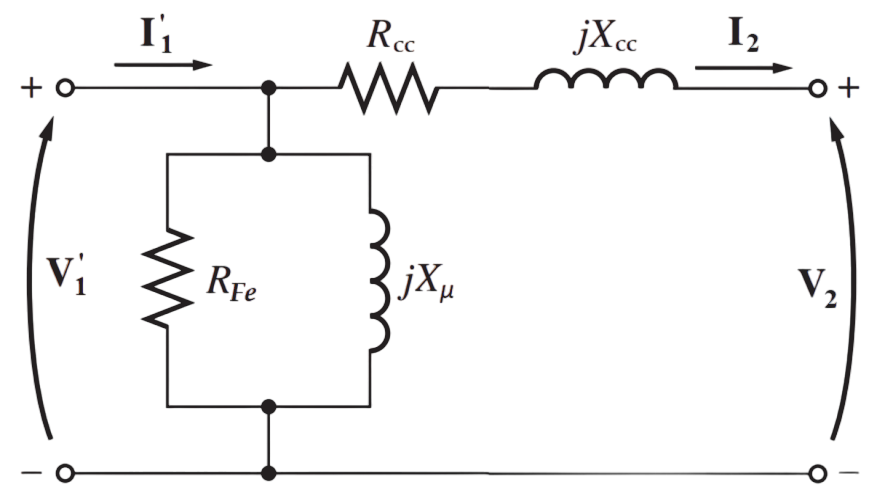
\includegraphics[width=\linewidth]{circuito-rv} \\
			
			\begin{tabular}{l l}
				Regulación de voltaje & $RV=\dfrac{V_{20}-V_{2pc}}{V_{2pc}}$\\[.3cm]
				& $RV = \dfrac{\frac{V_{1n}}{m} - V_{2pc}}{V_{2pc}}$\\[.3cm]
				RV ideal & $RV = 0 \%$ \\[.1cm]
				Cargas resistivas e inductivas & $RV_L > RV_R > 0$ \\[.1cm]
				Cargas capacitivas & $RV_C < 0$ \\
			\end{tabular}\\
		\end{multicols}
		
		
		
		
		
		\subtitulo{Eficiencia \vspace{.1cm}} 
		\vspace{.3cm}
		
		\begin{tabular}{l l}
			\multicolumn{2}{c}{$\eta = \dfrac{P_{out}}{P_{in}}= \dfrac{S \cos(\phi)}{S \cos(\phi )+P_{fe}+P_{\mu}}$\vspace{.2cm}}\\
			
			Eficiencia máxima & $cos(\phi)=1$ y $ P_{fe}=P_{\mu }$ \\
			Potencia útil & $P_{out} = S \cos \phi$\\
			Potencia demandada & $P_{in} = P_{out} + P_{p}$\\
			Pérdidas en potencia & $P_p = P_{Fe} + P_\mu$\\
		\end{tabular}
		
		\vspace{.3cm}
		
		\subtitulo{Índice de Carga}
		\vspace{.3cm}
		
		\begin{tabular}{l l}
			$C = \dfrac{I}{I_n}$ & $C_{opt} = \sqrt{\dfrac{P_0}{P_{cc}}}$\\
		\end{tabular}
		
		
	
	
	
\end{cajita}
\end{document}